\documentclass[11pt]{article}
\usepackage[margin=2.4cm]{geometry}
\usepackage{amsmath,amssymb}
\usepackage{booktabs}
\usepackage{graphicx}
\usepackage{xcolor}
\usepackage[colorlinks=true,linkcolor=teal!50!black,urlcolor=teal!50!black]{hyperref}

\graphicspath{{../campaign/outputs/xy_phase_plane/}}

\newcommand{\Jzz}{J_{zz}}
\newcommand{\Jpm}{J_{\pm}}
\newcommand{\Jpmpm}{J_{\pm\pm}}
\newcommand{\gsix}{g_6}
\newcommand{\gfour}{g_4}
\newcommand{\Ohex}{O_{\rm hex}}
\newcommand{\Ofour}{O_{4}}
\newcommand{\Pice}{P_{\rm ice}}

\title{How the flux sector was determined on the $(J_x,J_y)$ plane\\
\large A methods record for the cubic-16 XYZ scan}
\author{}
\date{5 August 2026}

\begin{document}
\maketitle

\begin{abstract}
\noindent
This note records exactly how the $(J_x,J_y)$ phase diagrams were computed
and how the $0$-flux / $\pi$-flux label was assigned, including the two
things that make the answer non-obvious: the label cannot be read off the
raw cluster, and the winding-free label needs no counterterm.  The headline
numbers: the raw ground state reports positive hexagon flux in all $1681$
cells of the plane, whereas the winding-free (masked) ground multiplet
gives a flux that is quantised to $-1/4$, $+1/4$ or exactly zero, and is
nonzero \emph{if and only if} the protected ground multiplet is six-fold
degenerate.  Every validation, every failure and every caveat is listed.
\end{abstract}

%=====================================================================
\section{Model, parametrisation, and what was scanned}

The cubic-16 cluster of the pyrochlore lattice carries $16$ sites, $8$
tetrahedra, $36$ four-loops and $16$ contractible hexagons, with $90$
two-in--two-out (ice) configurations.  With $J_z\equiv\Jzz=1$ the
Hamiltonian at zero twist is linear in the two transverse couplings,
\begin{equation}
H \;=\; \underbrace{\tfrac12\sum_t \bigl(n^{\uparrow}_t-2\bigr)^2}_{\text{Ising}}
\;-\;\Jpm\!\!\sum_{\langle ij\rangle}\!\bigl(S^+_iS^-_j+{\rm h.c.}\bigr)
\;+\;\Jpmpm\!\!\sum_{\langle ij\rangle}\!\bigl(S^+_iS^+_j+{\rm h.c.}\bigr),
\label{eq:H}
\end{equation}
so the three pieces are assembled once and recombined per grid point.  The
scan is over the square $J_x,J_y\in[-1,1]$ at $J_z=1$ on a $41\times41$
grid, with the dominant-$a$ mapping
\begin{equation}
\Jpm=-\frac{J_x+J_y}{4},\qquad \Jpmpm=\frac{J_x-J_y}{4}.
\label{eq:map}
\end{equation}
The XXZ line of the earlier campaign is the diagonal $J_x=J_y$; the
$56$-cell $(\Jpm,\Jpmpm)$ campaign grid occupies a narrow diagonal band,
drawn as open circles on every panel.

Because $\Jpmpm\neq0$ breaks $S^z$ conservation, the working basis is the
full $2^{16}=65\,536$ spin basis, not a fixed-magnetisation block.

%=====================================================================
\section{The naive phase diagram}

\emph{Everything in \texttt{fig\_xy\_phase} and \texttt{fig\_xy\_flux} is
ordinary exact diagonalisation}: full spectrum, no ice projection, no mask,
no counterterm.  Per grid point the ten lowest levels are obtained with
\texttt{eigsh} and the ground state gives the ice weight
$Z=\langle\psi|\Pice|\psi\rangle$, the mean ice violation
$\langle\sum_t Q_t^2\rangle$, the gap, and the two loop amplitudes of
Sec.~\ref{sec:flux}.

\paragraph{A solver note that mattered.}  The first pass stalled: one point
consumed $8174$~s and four array tasks died on a three-hour wall or on
\texttt{ArpackNoConvergence}.  The cause was not iteration count but Krylov
space --- \texttt{eigsh(k=10)} defaults to \texttt{ncv}$=21$, far too tight
where the low levels are clustered below $10^{-4}$.  Setting
\texttt{ncv}$=80$ (escalating to $180$ and $300$), seeding with the
ice-uniform vector and warm-starting from the previous point reduced the
same points to $6$--$11$~s, a factor above $800$ on the worst one.  The
$861$-point upper triangle then completed in under ten minutes.

\paragraph{Missing cells.}  Of $164$ cells lost to the failed tasks, $74$
were recovered by the reflection of Sec.~\ref{sec:symmetry}, $82$ from the
per-point lines the dead tasks had already printed, and the remaining $8$
by re-solving; the final assembly uses no scraped values at all.  The
internal symmetry check returns $1.5\times10^{-13}$ on the gap and
$1.7\times10^{-12}$ on the ice violation.  It returns $2.9\times10^{-3}$ on
the ice weight, which is not bookkeeping error but the genuine eigenvector
ambiguity in the near-degenerate region; it is left visible rather than
removed by rebuilding the plane from one triangle.

%=====================================================================
\section{The flux observable}
\label{sec:flux}

The $0$-flux / $\pi$-flux label of a quantum spin ice is the sign of the
contractible hexagon amplitude.  For a hexagon $h$ with sites ordered
around the ring,
\begin{equation}
\Ohex^{(h)} \;=\; S^+_1S^-_2S^+_3S^-_4S^+_5S^-_6 \;+\; {\rm h.c.},
\qquad
\Ohex \;=\; \frac{1}{N_{\rm hex}}\sum_{h}\Ohex^{(h)},
\label{eq:ohex}
\end{equation}
with $N_{\rm hex}=16$ the contractible hexagons (those of zero winding).  In
the $S^z$ product basis $\Ohex^{(h)}$ is a permutation-like operator: it is
nonzero only on the two configurations in which spins alternate around the
ring, and it maps each to the other by flipping all six.  Including both
alternating patterns is what makes it Hermitian.  The same construction on
the $36$ wrap-around four-loops defines $\Ofour$, the finite-size artefact
amplitude.  Positive $\langle\Ohex\rangle$ is $0$-flux, negative is
$\pi$-flux.

\subsection{Why the raw cluster gets the sign wrong}

Measured on the raw ground state, $\langle\Ohex\rangle$ is
\emph{positive in all $1681$ cells}, ranging only over
$+0.013$ to $+0.123$: raw ED labels the entire plane $0$-flux and never
produces a $\pi$-flux signature anywhere.  That is an artefact, and its
mechanism is the one this project exists to remove.  The wrap-around
amplitude $\gfour=4\Jpm^2/\Jzz$ is \textbf{even} in $\Jpm$ while the
physical ring exchange $\gsix=12|\Jpm|^3/\Jzz^2$ is \textbf{odd}.  For
$\Jpm>0$ the two reinforce and the raw sign is accidentally right; for
$\Jpm<0$ --- every cerium pyrochlore --- they oppose, and on this cluster
the artefact wins.  Table~\ref{tab:xxz} shows the inversion directly, with
$\langle\Ofour\rangle$ sitting $3$--$6\times$ above $\langle\Ohex\rangle$
in the raw state and collapsing once the winding is removed.

\begin{table}[h]
\centering
\small
\begin{tabular}{rrrrrrr}
\toprule
& \multicolumn{3}{c}{naive ED} & \multicolumn{3}{c}{winding-free $H+C$}\\
\cmidrule(lr){2-4}\cmidrule(lr){5-7}
$\Jpm$ & $Z$ & $\langle\Ohex\rangle$ & $\langle\Ofour\rangle$
       & $Z$ & $\langle\Ohex\rangle$ & $\langle\Ofour\rangle$\\
\midrule
$-0.02$ & $0.962$ & $+0.115$ & $0.356$ & $0.986$ & $-0.248$ & $0.022$\\
$-0.05$ & $0.888$ & $+0.107$ & $0.348$ & $0.907$ & $-0.238$ & $0.056$\\
$-0.10$ & $0.735$ & $+0.091$ & $0.326$ & $0.692$ & $-0.209$ & $0.056$\\
$-0.15$ & $0.613$ & $+0.079$ & $0.307$ & $0.477$ & $-0.177$ & $0.058$\\
$-0.20$ & $0.525$ & $+0.069$ & $0.290$ & $0.326$ & $-0.149$ & $0.066$\\
$-0.25$ & $0.461$ & $+0.063$ & $0.278$ & $0.230$ & $-0.122$ & $0.092$\\
$-0.30$ & $0.415$ & $+0.058$ & $0.269$ & $0.172$ & $-0.067$ & $0.147$\\
$-0.35$ & $0.379$ & $+0.054$ & $0.261$ & $0.144$ & $-0.009$ & $0.178$\\
$+0.046$ & $0.723$ & $+0.119$ & $0.335$ & $0.752$ & $+0.215$ & $0.193$\\
\bottomrule
\end{tabular}
\caption{The XXZ line.  Naive ED reports $0$-flux at every coupling; the
winding-free state is $\pi$-flux throughout $\Jpm<0$, with the magnitude
decaying as the band dissolves.  Naive ED also overstates the ice weight
once $|\Jpm|>0.1$, because the artefact binds the ice manifold more tightly
than the physics does.}
\label{tab:xxz}
\end{table}

\subsection{Attribution: the operator is right, the state was wrong}

Before accepting that reading, the discrepancy was localised.  The raw
full-basis measurement was reproduced with the \emph{reference} code path
--- the $S^z=0$ translation-sector basis and the counterterm campaign's own
\texttt{loop\_expectation} --- on the bare Hamiltonian.  At $\Jpm=-0.10$
both give $E=-0.502949$, gap $0.10603$, $Z=0.7346$,
$\langle\Ohex\rangle=+0.0914$, $\langle\Ofour\rangle=+0.3264$, agreeing to
every printed digit.  The Hamiltonian conventions were checked to match as
well (\texttt{amplitude}$=-\Jpm\times$phase in both).  The entire gap to the
cached $-0.209$ is therefore $H$ versus $H+C$: a difference of state, not a
bug in the observable.

%=====================================================================
\section{The winding-free determination}

\subsection{The mask, and what it is applied to}

Splitting the Hilbert space with $P=\Pice$ (rank $90$) and $Q=1-P$ (rank
$65\,446$) and eliminating $Q$ exactly gives the Feshbach map
\begin{equation}
F(z) \;=\; PHP \;+\; \underbrace{PHQ\,(z-QHQ)^{-1}QHP}_{\Sigma(z)},
\label{eq:feshbach}
\end{equation}
whose self-consistent roots $E=\mathrm{eig}\,F(E)$ are exact eigenvalues of
$H$ with nonzero ice weight.  \textbf{The mask deletes every entry of
$F(z)$ connecting different transport (polarisation) sectors.}  It is one
operation, \texttt{sector\_project} in
\texttt{DownfoldBlocks.f\_matrix}.

It is worth being explicit about what the mask is \emph{not}, because the
natural guess is wrong.  It is not the deletion of cross-sector matrix
elements of $H$: the ice block $PHP$ is diagonal, so there are no such
elements to delete.  Every winding amplitude is generated by excursions
through the spinon space and therefore lives entirely in the self-energy
$\Sigma(z)$.  Deleting entries of $H$ would accomplish nothing; deleting
them from the fold is the whole method.

\subsection{Why no counterterm is involved}

The counterterm $C=-\bigl(\text{transport-changing part of }F(z_0)\bigr)$,
supported inside the ice manifold, is the operator that makes $H+C$ a
genuine Hamiltonian on the full space whose fold equals the masked map at
the anchor $z_0$.  It exists because the masked map returns energies and
ice-block vectors but no states above the band and no full-space
wavefunctions --- and it is exact only at $z_0$, which is the origin of the
residual $z$-dependence of order $1-Z$.

None of that is needed here.  A contractible hexagon flip takes an ice
configuration to an ice configuration, so $\Ohex$ closes inside the
$90$-dimensional manifold and is a dense $90\times90$ matrix in the ice
basis.  The masked map's own ground multiplet is therefore sufficient, and
the flux reported below is computed with the mask alone.

\subsection{Extraction, step by step}

At each grid point:
\begin{enumerate}\itemsep2pt
\item build $H$ from Eq.~(\ref{eq:H}) on the full $65\,536$ basis at the
$(\Jpm,\Jpmpm)$ of Eq.~(\ref{eq:map});
\item block-diagonalise and fold, obtaining $PHP$, the poles
$\{\varepsilon_q\}$ of $QHQ$ and the rotated coupling
(Sec.~\ref{sec:klein});
\item solve $E=\mathrm{eig}\,\Delta[F(E)]$ for all $90$ branches by
guaranteed bisection, where $\Delta$ is the sector mask.  A branch with no
root below the lowest pole has migrated into the continuum and is counted
as lost --- that count is the band-completeness diagnostic, not an error;
\item take the lowest root $E_0$ and the multiplet of branches within
$10^{-9}$ of it; diagonalise $\Delta[F(E_0)]$ and keep those eigenvectors
$\{\phi_m\}$;
\item report $\langle\Ohex\rangle=\frac{1}{M}\sum_m\phi_m^\dagger \Ohex
\phi_m$ and the ice weight
$Z=\frac{1}{M}\sum_m\bigl[1-\phi_m^\dagger\,\partial_z\Sigma(E_0)\,
\phi_m\bigr]^{-1}$.
\end{enumerate}

\paragraph{Averaging over the multiplet is mandatory.}  The masked ground
state is degenerate by theorem, not by accident: the sector structure
protects a multiplicity of six at weak coupling and two after it
reorganises.  A single eigenvector of a degenerate subspace is whatever
LAPACK returned, so every expectation value is averaged over the multiplet.
The spread across multiplet members is recorded and is below $10^{-6}$
(typically $10^{-31}$) at \emph{all} $379$ points with a surviving band, so
the averaging changes no value while removing the basis dependence.

%=====================================================================
\section{Numerics}
\label{sec:klein}

The one expensive step is the eigendecomposition of $QHQ$.  On the full
basis that is a single dense solve of dimension $65\,446$, which not only
costs $\sim9$~h but \emph{segfaults}: $n^2=4.3\times10^9$ exceeds $2^{31}$
and overflows LAPACK's \texttt{int32} indexing.  It is not a memory
problem and no amount of RAM fixes it.

\subsection{The Klein group}

The pyrochlore cubic cell contains four FCC primitive cells, so four
translations map the $16$-site cluster to itself:
\begin{equation}
t_0=(0,0,0),\quad t_1=\bigl(0,\tfrac12,\tfrac12\bigr),\quad
t_2=\bigl(\tfrac12,0,\tfrac12\bigr),\quad
t_3=\bigl(\tfrac12,\tfrac12,0\bigr),
\end{equation}
in units of the cubic edge.  Each doubles to a cubic lattice vector, so
$t_i^2=\mathbb{1}$ on the cluster, and the product of any two distinct
non-identity translations is the third, $t_1t_2=t_3$.  The group is
therefore $\mathbb{Z}_2\times\mathbb{Z}_2$ --- the Klein four-group $V_4$,
not the cyclic $\mathbb{Z}_4$ --- and this is what the ``Klein'' in
\texttt{build\_blocks\_klein} refers to.  All four irreps are
one-dimensional with characters $\pm1$, labelled $++$, $+-$, $-+$, $--$.

Two facts make it usable.  Both terms of Eq.~(\ref{eq:H}) are translation
invariant, so all four elements commute with $H$ at \emph{any}
$(\Jpm,\Jpmpm)$ --- the blocking survives switching on the pair term, which
is what breaks $S^z$ and forces the full basis in the first place.  And the
ice manifold is closed under them, so the $P/Q$ split commutes with the
decomposition.  Hence $QHQ$ block-diagonalises into four blocks of
$\approx16\,384$: the flop count falls by $\sim16\times$ (four solves of
$n/4$ against one of $n$), peak memory from $\sim100$~GB to $\sim10$~GB,
and each block has $n^2=2.7\times10^8$, comfortably inside \texttt{int32}.

Within each irrep $k$ the ice components are $I_k=B_k[\text{ice}]^\dagger$,
of size $m_k\times90$; an SVD gives an orthonormal $O_k$ of rank $d_k$ with
$\sum_k d_k=90$.  Projecting the ice subspace out,
$(1-O_kO_k^\dagger)H_k(1-O_kO_k^\dagger)$, leaves $d_k$ \emph{spurious}
ice-kernel modes alongside the genuine $QHQ$ poles.  These must be
separated by their overlap with $O_k$ and \textbf{not} by eigenvalue, since
genuine poles cross zero at strong coupling and an eigenvalue threshold
would discard real physics.

That classification is precisely what fails at the four unresolved points
below: the overlaps stop being bimodal, so no threshold separates $36$
genuine from the $38$--$47$ modes that look spurious.  The Klein
decomposition itself is exact; it is the heuristic that sorts its output
which breaks.

Cost: $174$~s per point on an H100 against $2600$~s on $16$ CPU cores, so
the production run used GPUs --- $861$ points over $20$ array tasks,
$3$~h~$52$~m wall.  Results are checkpointed after every point and the
script resumes from disk, so a wall-clock overrun costs one point rather
than a task.

\paragraph{Four points did not resolve.}  The ice-kernel classification
failed at $(J_x,J_y)=(-1,+1)$, $(-0.75,+1)$, $(0,+1)$ and $(+1,+1)$, with
between $38$ and $47$ modes looking spurious against an SVD rank of $36$
and overlap ranges reaching from $\sim10^{-31}$ (or exactly $0$) to $1$.
All four sit on the $J_y=+1$ boundary at maximal coupling, where extra
degeneracy makes the overlaps ambiguous; the failure is a limitation of the
classification heuristic, not of the mask.  They are recorded as
unresolved and left blank.

\subsection{Symmetries not yet exploited}
\label{sec:unused}

The Klein decomposition is the only reduction currently implemented, and it
is not the only one available.  All of the following are exact at any
$(\Jpm,\Jpmpm)$ unless stated.

\paragraph{$U(1)$ (XXZ line only).}  At $\Jpmpm=0$ total $S^z$ is
conserved and the problem lives in the $12\,870$-state $S^z=0$ block,
which is why the counterterm campaign was inexpensive along the line.  The
pair term destroys it, so this buys nothing off the diagonal.

\paragraph{$\mathbb{Z}_2$ parity (everywhere), worth $8\times$.}  The pair
term shifts $N_\uparrow$ by $\pm2$ and the exchange preserves it, so
$\Pi=(-1)^{N_\uparrow}$ commutes with $H$ for all couplings.  Every ice
state has $N_\uparrow=8$ exactly --- each site belongs to exactly one
A-tetrahedron, so summing the ice rule over the four A-tetrahedra gives
$4\times2=8$ --- hence $P$ lies entirely in the even sector, and
$\Sigma(z)=PHQ(z-QHQ)^{-1}QHP$ cannot reach the odd sector at any order.
The $32\,768$ odd states are therefore not a block to be diagonalised
separately but irrelevant, and can be dropped: $QHQ$ falls from $65\,446$
to $32\,678$, the Klein blocks from $\approx16\,362$ to $\approx8\,170$.

\begin{table}[h]
\centering
\small
\begin{tabular}{lrrrr}
\toprule
reduction & blocks & dimension & relative flops & memory/block\\
\midrule
none (direct) & $1$ & $65\,446$ & --- & \emph{int32 overflow}\\
Klein $V_4$ (implemented) & $4$ & $16\,362$ & $1$ & $2.14$~GB\\
$+$ parity & $4$ & $8\,170$ & $1/8$ & $534$~MB\\
$+$ global spin flip & $8$ & $4\,085$ & $1/32$ & $134$~MB\\
\bottomrule
\end{tabular}
\caption{Available reductions of $QHQ$.  Parity is exact and nearly free to
implement: restrict the basis before building anything and the existing
Klein path runs unchanged.  At $174$~s per point, the parity factor alone
would bring the full plane from $\sim42$ to $\sim6$ GPU-hours --- and would
have made the abandoned CPU route viable at $\sim325$~s per point.}
\label{tab:reductions}
\end{table}

\paragraph{Global spin flip (everywhere), worth a further $4\times$.}
$X=\prod_i\sigma^x_i$ commutes with all three terms of Eq.~(\ref{eq:H}),
preserves the ice manifold and $N_\uparrow$ parity, and leaves
$\Ohex+\mathrm{h.c.}$ invariant.  It is more invasive than parity: it
\emph{permutes} the polarisation sectors ($p\to-p$) rather than fixing
them, so it interacts with the mask's sector labelling and with the
SVD-based ice-kernel separation --- the one step that already fails at four
points.  Worth taking, but as a separately validated exercise, not as part
of the same change.

\paragraph{Validation any such change must pass.}  Re-solve points that
already exist and require agreement to machine precision.  The flux is
quantised at $\pm1/4$ and so is insensitive to small errors; the ice weight
and the band gap are the discriminating checks.

%=====================================================================
\section{The exchange symmetry, and its verification}
\label{sec:symmetry}

$J_x\leftrightarrow J_y$ sends $\Jpmpm\to-\Jpmpm$ at fixed $\Jpm$ and is an
exact symmetry, implemented by the diagonal transformation
$D=i^{N_\uparrow}$: the pair term picks up $i^{\pm2}=-1$ while the exchange
term, which conserves $N_\uparrow$, is untouched.  The hexagon operator has
three $S^+$ and three $S^-$, hence $i^3(-i)^3=1$, and is invariant.  Only
the upper triangle therefore needs solving: $861$ points cover all $1681$
cells.

This was verified rather than assumed, and the check had to be designed
with some care --- the assembled figure writes both $(i,j)$ and $(j,i)$
from one solve, so a symmetry check computed from it returns zero by
construction and means nothing.  Instead both members of six mirror pairs
(with $\Jpmpm=\pm0.25$, genuinely different matrices) were solved
independently.  They agree \emph{bitwise} in energy, gap, ice weight, ice
violation, hexagon flux and winding amplitude --- as expected when the
symmetry acts by a diagonal similarity, since Lanczos from the same real
seed then builds an identical tridiagonal matrix.

%=====================================================================
\section{Results}

\subsection{Three phases, and a quantised label}

\begin{table}[h]
\centering
\small
\begin{tabular}{lrrl}
\toprule
region & upper triangle & full plane & ground multiplet\\
\midrule
$\pi$-flux, $\langle\Ohex\rangle=-1/4$ & $101$ & $193$ & six-fold\\
$0$-flux, $\langle\Ohex\rangle=+1/4$ & $16$ & $29$ & six-fold\\
no ring resonance, $\langle\Ohex\rangle=0$ & $262$ & $497$ & one-, two- (or $90$-)fold\\
no ice-descended band & $478$ & $962$ & ---\\
unresolved & $4$ & $7$ & ---\\
\midrule
total & $861$ & $1681$ & \\
\bottomrule
\end{tabular}
\caption{Winding-free classification of the plane.  Only $13\%$ of the
plane carries a flux at all, and the overwhelming majority of that is
$\pi$ --- the label naive ED never produces anywhere.}
\label{tab:phases}
\end{table}

Two features are sharper than expected.  First, the flux is
\textbf{quantised}: among all resonant cells the magnitude takes the single
value $|\langle\Ohex\rangle|=0.25$, with the individual numbers equal to
$\pm1/4$ to $10^{-16}$ and nothing in between.  Second, the resonant set
coincides \emph{exactly}, cell by cell, with the set where the protected
ground multiplet is six-fold: all $117$ six-fold cells are resonant, and
all $262$ cells of multiplicity $1$, $2$ or $90$ have zero flux.  The
protected multiplet is what carries the flux; where the protection is lost,
the resonance is gone with it.

A value of exactly $1/4$ is what a uniform-amplitude resonance over the ice
manifold would give: with the normalisation of Eq.~(\ref{eq:ohex}),
$\langle\Ohex\rangle$ for an equal-amplitude state equals
$\langle n_{\rm flip}\rangle/N_{\rm hex}$, so $1/4$ corresponds to a mean of
exactly four flippable hexagons per ice configuration.  That reading is
consistent with the measurement but has not been verified here, and is
offered as an interpretation only.

\subsection{Naive against winding-free}

The two diagrams disagree about the plane at the coarsest level, not in
detail.  Naive ED returns a confident ice weight, gap and positive flux in
every one of the $1681$ cells.  The winding-free map says that $57\%$ of
the plane has no ice-descended band at all, a further $30\%$ has a band
carrying no hexagon resonance, and the $13\%$ that does carry a flux is
mostly $\pi$.  The disagreement over the \emph{existence} of the band is
arguably the more important of the two.

The winding-free diagram also reproduces, by an independent route, the
dissolution threshold found in the $\Jpmpm$ study: the campaign cell
$(\Jpm,\Jpmpm)=(-0.05,0.30)$ maps to $(J_x,J_y)=(0.7,-0.5)$ and lands in
the no-band region, consistent with the band dying once
$\Jpmpm/|\Jpm|\gtrsim5$.  A substantial number of the $56$ campaign cells
lie in the no-resonance region rather than in the $\pi$-flux disc.

\begin{figure}[h]
\centering
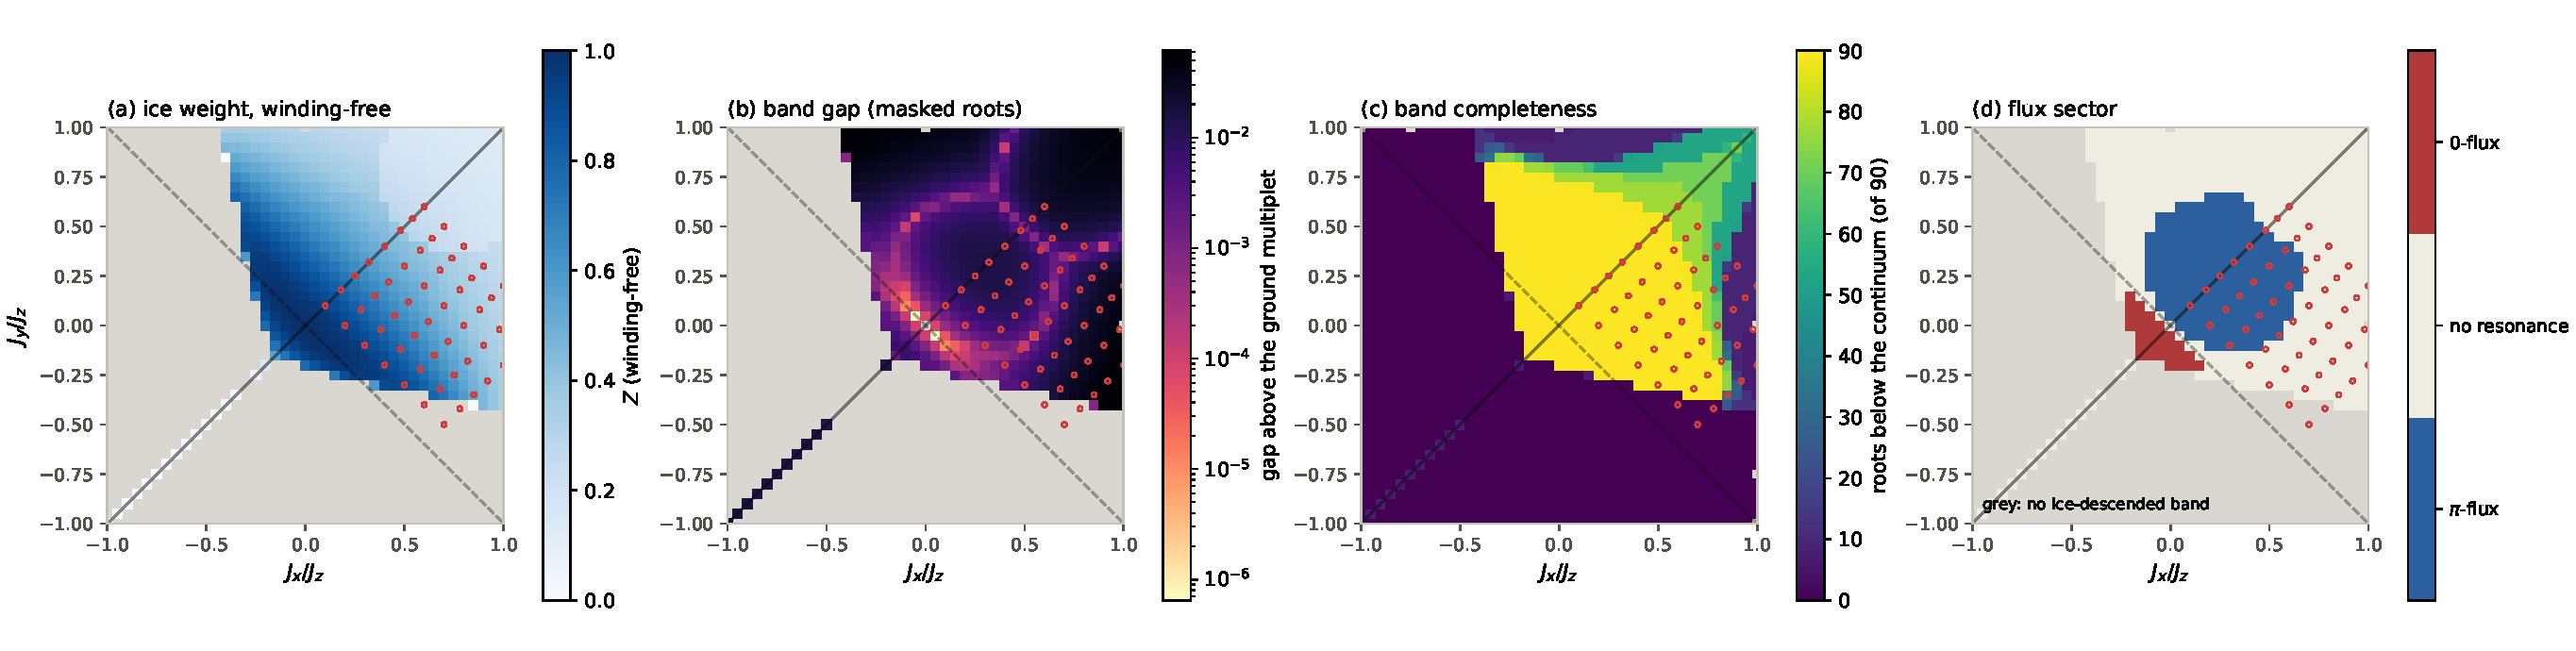
\includegraphics[width=\textwidth]{fig_xy_masked.pdf}
\caption{The winding-free plane.  (a) ice weight of the masked ground
multiplet; (b) gap above the protected multiplet \emph{within the
ice-descended band} --- not the same object as the naive full-spectrum gap,
and not to be compared with it; (c) band completeness, roots surviving out
of $90$; (d) flux sector, categorical.  Grey is ``no ice-descended band''.
The ring of near-degeneracies in (b), encircling the origin at roughly the
boundary of the $\pi$-flux disc, is an observation from the data and has
not been identified here.}
\end{figure}

%=====================================================================
\section{What is not established}

\begin{itemize}\itemsep2pt
\item \textbf{The naive ice-violation panel has no winding-free
counterpart.}  $\langle\sum_t Q_t^2\rangle$ requires the full-space
wavefunction, which is exactly what the masked map does not carry and what
the counterterm exists to supply.  Band completeness occupies that panel
instead.
\item \textbf{Panel (b) is a different quantity} from the naive gap panel:
the gap above the protected multiplet inside the band, versus the gap of
the full spectrum.  They are labelled separately and should not be
overlaid.
\item \textbf{The masked flux is an ice-manifold expectation}, taken on the
normalised $90$-dimensional vector, whereas the cached $H+C$ numbers are
full-state expectations; the two are related by
$\langle\psi|\Ohex|\psi\rangle = Z\langle\phi|\Ohex|\phi\rangle +
(\text{$Q$ terms})$.  At $\Jpm=-0.10$, $0.692\times0.25=0.173$ against a
cached $-0.209$, leaving $-0.036$ from the spinon dressing; at $+0.046$,
$0.752\times0.25=0.188$ against $+0.215$.  Signs agree and residuals are of
the expected size, but the two conventions are not interchangeable.
\item \textbf{Four boundary points are unresolved} and are not
extrapolated over.
\item \textbf{The $1/4$ interpretation} of the preceding section is a
conjecture, not a derivation.
\item \textbf{One cluster.}  Everything here is cubic-16; nothing in this
note addresses the thermodynamic limit, and the cluster is the error bar.
\end{itemize}

%=====================================================================
\section{Reproduction}

\begin{table}[h]
\centering
\small
\begin{tabular}{ll}
\toprule
file & role\\
\midrule
\texttt{campaign/scan\_xy\_phase\_plane.py} & naive ED over the plane, one task per column\\
\texttt{campaign/scan\_xy\_points.py} & naive ED at a point list, with the \texttt{ncv} ladder\\
\texttt{campaign/fill\_xy\_phase\_gaps.py} & reflection, log recovery, assembly of the naive plane\\
\texttt{campaign/scan\_xy\_masked\_flux.py} & masked Feshbach map, flux and ice weight\\
\texttt{campaign/check\_flux\_symmetry.py} & mirror-pair test of $J_x\leftrightarrow J_y$\\
\texttt{campaign/make\_xy\_phase\_figure.py} & naive plane, three panels\\
\texttt{campaign/make\_xy\_flux\_figure.py} & naive flux, artefact, and the XXZ inversion\\
\texttt{campaign/make\_xy\_masked\_figure.py} & winding-free plane, four panels\\
\texttt{campaign/make\_naive\_vs\_wf\_figure.py} & the XXZ-line contrast of Table~\ref{tab:xxz}\\
\texttt{src/qsi\_campaign/downfold.py} & \texttt{build\_blocks\_klein}, \texttt{solve\_roots}, the mask\\
\bottomrule
\end{tabular}
\end{table}

\noindent
Production jobs: naive plane \texttt{18332139} (plus the repair chain),
naive flux \texttt{18341289}/\texttt{18341649}, mirror check
\texttt{18341657}, winding-free plane \texttt{18365005}.  Raw records are
\texttt{campaign/outputs/xy\_phase\_plane/\{xyscan,flux\_points,masked\_flux\}\_*.json};
the masked records carry both the masked and unmasked fold at every point,
so the winding contribution can be isolated within one framework without
changing basis, solver or normalisation.

\end{document}
